%
% Library Document for ACM/ICPC
% LaTeX based on library by kaicho-@IHI (U-Tokyo)
%

\documentclass[10pt]{jsarticle}
\usepackage[left=3cm,right=2cm,top=4cm,bottom=3cm]{geometry}
\usepackage{multicol}
\usepackage{amsmath}
\usepackage{eclbkbox}
\usepackage{fancybox}
\usepackage{pifont}
\usepackage{txfonts}
\usepackage{picins}
\usepackage{ascmac}
\usepackage{graphicx}
\usepackage{color}
\usepackage{listings,jlisting}

\newcommand{\codesize}{\footnotesize}

\lstset{%
 language={C++},
 backgroundcolor={\color[gray]{.90}},%
 basicstyle={\codesize\ttfamily},%
 identifierstyle={\codesize},%
 commentstyle={\codesize\itshape},%
 keywordstyle={\codesize\bfseries},%
 ndkeywordstyle={\codesize},%
 stringstyle={\codesize\ttfamily},
 frame={tblr},%
 breaklines=true,%
 columns=[l]{fullflexible},%
 tabsize=4,%
% numbers=left,%
 xrightmargin=0zw,%
 xleftmargin=0zw,%
 numberstyle={\scriptsize},%
 stepnumber=1,
 numbersep=1zw,%
 lineskip=-0.5ex%
}

%\everymath{\displaystyle}
\newenvironment{code}%
 {\VerbatimEnvironment\begin{breakbox}\vspace{-1em}\footnotesize\begin{Verbatim}}%
 {\end{Verbatim}\vspace{-.8em}\end{breakbox}}

\setlength{\columnseprule}{0.2pt}

\addtolength{\oddsidemargin}{-.5cm}
\addtolength{\voffset}{-1.2cm}
\addtolength{\textwidth}{1cm}
\addtolength{\textheight}{2cm}
\setlength{\fboxsep}{.7em}
\renewcommand{\breakboxskip}{.7em}
\renewcommand{\ttdefault}{pcr}
\renewcommand{\vec}[1]{\boldsymbol{#1}}
%\newcommand{\accepted}[1]{\ding{52} Accepted (#1)}
%\newcommand{\nottested}[0]{\ding{56} NOT TESTED!}
\newcommand{\accepted}[1]{}
\newcommand{\nottested}[0]{}
\newcommand{\derived}[1]{\ding{224} Derived from #1}
\newcommand{\todo}[1]{\textbf{TODO: #1}}
\newcommand{\mymaketitle}[3]%
 {\begin{center}\begin{tabular}{lr}\textsf{\huge #1}\hspace{3.5cm}\mbox{}&#3\\\hline&#2\end{tabular}\end{center}}
\DeclareMathOperator{\vers}{vers}
\setcounter{tocdepth}{3}
\newcommand{\w}[1]{\textbf{#1}}

\makeatletter
\def\@oddhead{\hfill\thepage}
\def\@oddfoot{}
\def\@evenhead{\hfill\thepage}
\def\@evenfoot{}
\def\ps@titlepage{\let\@oddhead\@empty}
\makeatother


% fate test

\makeatletter
\let\@@shipout\shipout
\def\shipout\vbox{\@@shipout\vbox\bgroup\afterassignment\insertBackGround\let\reserved@a=}
\def\insertBackGround#1{#1%
        \iftombow
                \copy\BackGround\kern0pt
        \else
                \kern-1truein\moveleft1truein\copy\BackGround\kern1truein
        \fi}
\newbox\BackGroundUnit
\newbox\BackGround
\setbox\BackGroundUnit\hbox{\includegraphics*[bb=7 0 355 500,width=21cm]{fatebg.png}}
\@tempdima\paperheight
\advance\@tempdima\ht\BackGroundUnit\advance\@tempdima\dp\BackGroundUnit
\setbox\BackGround\vbox to \@tempdima{
        \@tempdima=\paperwidth\advance\@tempdima\wd\BackGroundUnit
        \leaders\hbox to\@tempdima{\leaders\copy\BackGroundUnit\hfil}\vfil
}
\wd\BackGround=0pt\ht\BackGround=0pt\dp\BackGround=0pt
\makeatother



\begin{document}

\mymaketitle{ここのところのリファレンス}{by kkntkr / unknown}%
{Last Update: 2008/09/12}

\vspace{0.2cm}
\begin{center}
\doublebox{にょろーんの精神でがんばってください --- 桜庭 俊}
\end{center}
\vspace{0.2cm}


\begin{multicols}{2}

\setcounter{section}{-1}

\section{基礎}

\subsection{いつものマクロ}

\begin{lstlisting}
#define REP(i,n) for(int i = 0; i < (int)(n); i++)
#define FOR(i,c) for(__typeof((c).begin()) i = (c).begin(); i != (c).end(); ++i)
#define ALLOF(c) (c).begin(), (c).end()
\end{lstlisting}


\subsection{間違ったかな?と思ったら}

\begin{itemize}
\item{\w{とりあえず深呼吸。}}
\item{\w{これフローじゃね?}}
\item{\w{これ二分探索じゃね?}}
\item{\w{これ凸じゃね?}}
\item{\w{最小/最大/特異ケースのテスト}}
\item{-Wall, -Wextraはつけているか?}
\item{問題の条件をよみなおせ!}
\item{入力の形式はあっているか?}
\begin{itemize}
\item{入力ファイルを修正してそのままにしていないか}
\item{スペースを含む文字列}
\item{0-origin, 1-origin}
\item{(i,j) $<$-$>$ (x,y) 変換をはじめとする座標変換}
\item{改行コードwww}
\end{itemize}
\item{出力の形式はあっているか?}
\begin{itemize}
\item{スペルミス}
\item{-0.000}
\item{空行のはさみ方}
\item{デバッグ出力の削りのこし}
\item{解が無い時}
\end{itemize}
\item{オーバーフロー}
\begin{itemize}
\item{答えがintに収まらない}
\item{numeric\_limits$<$int$>$::max() * 2}
\item{bool型の変数にint/doubleを代入、関数の返り値型がbool (特に、DP/メモの型を後で変更した場合)}
\end{itemize}
\item{ポインタの進め忘れ}
\item{参照/イテレータの無効化}
\item{実数}
\begin{itemize}
\item{EPSを使わずに比較していないか}
\item{問題に合ったEPSの設定}
\item{NaN (/, sqrt, asin, acos, etc...)}
\end{itemize}
\item{switch}
\begin{itemize}
\item{breakし忘れていないか}
\item{defaultにassert(false)}
\end{itemize}
\item{ライブラリ関数}
\begin{itemize}
\item{全順序関係でないようなoperator$<$を使ったソート}
\item{accumulate/inner\_productの初期値は必ず型をキャストで明示すること}
\end{itemize}
\item{配列}
\begin{itemize}
\item{サイズは十分か?}
\item{初期化を忘れていないか?}
\item{番兵のせいでサイズ・インデックス・初期化が間違っていないか?}
\item{添字を間違っていないか?(jと書くべきところにi、など)}
\end{itemize}
\item{コピペ}
\begin{itemize}
\item{コピペ修正ミスは無いか?(y += dx みたいな)}
\end{itemize}
\item{考え方}
\begin{itemize}
\item{問題を分解したときに独立にとけないこともあるので柔軟に考えるといいよ}
\end{itemize}
\end{itemize}


%\vfill

%\begin{center}
%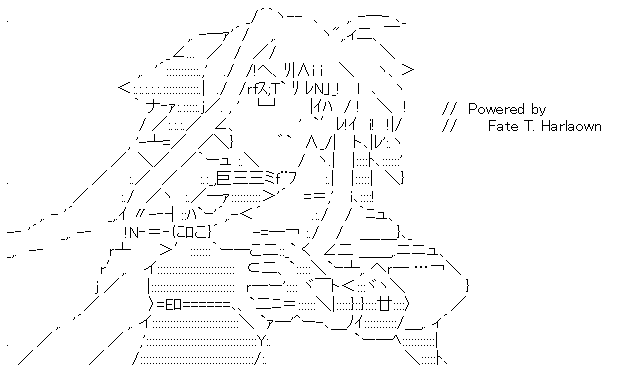
\includegraphics[width=0.98\hsize]{fate2-aa.eps}
%\end{center}

\newpage


\section{幾何}

\subsection{基礎}

\begin{lstlisting}
typedef complex<double> P;
struct L { P pos, dir; };
typedef vector<P> G;
struct C { P p; double r; };

inline double inp(const P& a, const P& b) {
  return (conj(a)*b).real();
}
inline double outp(const P& a, const P& b) {
  return (conj(a)*b).imag();
}

inline int ccw(const P& p, const P& r, const P& s) {
  P a(r-p), b(s-p);
  int sgn = signum(outp(a, b));
  if (sgn != 0)
    return sgn;
  if (a.real()*b.real() < -EPS || a.imag()*b.imag() < -EPS)
    return -1;
  if (norm(a) < norm(b) - EPS)
    return 1;
  return 0;
}

// ベクトルpをベクトルbに射影したベクトルを計算する
inline P proj(const P& p, const P& b) {
  return b*inp(p,b)/norm(b);
}
// 点pから直線lに引いた垂線の足となる点を計算する
inline P perf(const L& l, const P& p) {
  L m = {l.pos - p, l.dir};
  return (p + (m.pos - proj(m.pos, m.dir)));
}
// 線分sを直線bに射影した線分を計算する
inline L proj(const L& s, const L& b) {
   return (L){perf(b, s.pos), proj(s.dir, b.dir)};
}
\end{lstlisting}


\subsection{面積・体積}

\subsubsection{多角形の面積}

\begin{lstlisting}
double area(G& g) {
  int n = g.size();
  double s = 0.0;
  for(int i = 0; i < n; i++) {
    int j = (i+1)%n;
    s += outp(g[i], g[j])/2;
  }
  return abs(s);
}
\end{lstlisting}


\subsubsection{円と円の交差面積}

\begin{lstlisting}
double cc_area(const C& c1, const C& c2) {
  double d = abs(c1.p - c2.p);
  if (c1.r + c2.r <= d + EPS) {
    return 0.0;
  } else if (d <= abs(c1.r - c2.r) + EPS) {
    double r = c1.r <? c2.r;
    return r * r * PI;
  } else {
    double rc = (d*d + c1.r*c1.r - c2.r*c2.r) / (2*d);
    double theta = acos(rc / c1.r);
    double phi = acos((d - rc) / c2.r);
    return c1.r*c1.r*theta + c2.r*c2.r*phi - d*c1.r*sin(theta);
  }
}
\end{lstlisting}



\subsection{交差}


\subsubsection{各種交差判定}

\begin{lstlisting}
bool ls_intersects(const L& l, const L& s) {
  return (signum(outp(l.dir, s.pos-l.pos)) *
      signum(outp(l.dir, s.pos+s.dir-l.pos)) <= 0);
}
bool sp_intersects(const L& s, const P& p) {
  return ( abs(s.pos - p) + abs(s.pos + s.dir - p) - abs(s.dir) < EPS );
}
bool ss_intersects(const L& s, const L& t) {
  return (ccw(s.pos, s.pos+s.dir, t.pos) *
      ccw(s.pos, s.pos+s.dir, t.pos+t.dir) <= 0 &&
      ccw(t.pos, t.pos+t.dir, s.pos) *
      ccw(t.pos, t.pos+t.dir, s.pos+s.dir) <= 0);
}
\end{lstlisting}


\subsubsection{多角形と点の包含判定}

辺と点が重なれば包含。そうでなければ、
$\mathrm{abs}(\sum_i \arg((g_{i+1}-p)/(g_i-p))) > 1$ なら包含。


\subsubsection{円と円の交点}

\w{交点が0個または無限個だとうまく動かない。}

\begin{lstlisting}
pair<P, P> cc_cross(const C& c1, const C& c2) {
  double d = abs(c1.p - c2.p);
  double rc = (d*d + c1.r*c1.r - c2.r*c2.r) / (2*d);
  double rs = sqrt(c1.r*c1.r - rc*rc);
  P diff = (c2.p - c1.p) / d;
  return make_pair(c1.p + diff * P(rc, rs), c1.p + diff * P(rc, -rs));
}
\end{lstlisting}



\subsubsection{円と直線の交点}

\begin{lstlisting}
vector<P> cl_cross(const C& c, const L& l) {
  P h = perf(l, c.p);
  double d = abs(h - c.p);
  vector<P> res;
  if(d < c.r - EPS){
  P x = l.dir / abs(l.dir) * sqrt(c.r*c.r - d*d);
  res.push_back(h + x);
  res.push_back(h - x);
  }else if(d < c.r + EPS){
  res.push_back(h);
  }
  return res;
}
\end{lstlisting}


\subsubsection{凸多角形と線分の包含判定}

線分と凸多角形が内部で交差しているか判定する。接しているだけの場合には交
差しているとみなさない。

\w{多角形は凸でなければいけない。}
\w{多角形は反時計回りに与えられなければならない。}

\begin{lstlisting}
bool cgs_contains_exclusive(G& r, P from, P to) {
  int m = r.size();

  P dir0 = to - from;

  double lower = 0.0, upper = 1.0;
  REP(i, m) {
    int j = (i+1)%m;
    P a = r[i], b = r[j];
    P ofs = a - from;
    P dir1 = b - a;
    double num = (conj(ofs)*dir1).imag();
    double denom = (conj(dir0)*dir1).imag();
    if (abs(denom) < EPS) {
      if (num < EPS)
        lower = upper = 0.0;
    }
    else {
      double t = num / denom;
      if (denom > 0)
        upper <?= t;
      else
        lower >?= t;
    }
  }

  return (upper-lower > EPS);
}
\end{lstlisting}


\subsubsection{直線と直線の交点}

\w{直線が並行となるときに注意すること。}
\verb|denom| = 0 となるケース、すなわち\w{直線が平行となるとき}に注意すること。
\w{片方または両方が線分のとき}に使用する場合は、\verb|{ls,ss}_intersects()|等と併用して、交点がvalidなものか確認すること。

\begin{lstlisting}
P line_cross(const L& l, const L& m) {
  double num = outp(m.dir, m.pos-l.pos);
  double denom = outp(m.dir, l.dir);
  return P(l.pos + l.dir*num/denom);
}
\end{lstlisting}


\subsection{距離}


\subsubsection{各種距離}

\begin{lstlisting}
double lp_distance(const L& l, const P& p) {
  return abs(outp(l.dir, p-l.pos) / abs(l.dir));
}
double ll_distance(const L& l, const L& m) {
  return (ll_intersects(l, m) ? 0 : lp_distance(l, m.pos));
}
double ls_distance(const L& l, const L& s) {
  if (ls_intersects(l, s))
    return 0;
  return min(lp_distance(l, s.pos), lp_distance(l, s.pos+s.dir));
}
double sp_distance(const L& s, const P& p) {
  const P r = perf(s, p);
  const double pos = ((r-s.pos)/s.dir).real();
  if (-EPS <= pos && pos <= 1 + EPS)
    return abs(r - p);
  return min(abs(s.pos - p),
         abs(s.pos+s.dir - p));
}
double ss_distance(const L& s, const L& t) {
  if (ss_intersects(s, t))
    return 0;
  return (sp_distance(s, t.pos) <?
      sp_distance(s, t.pos+t.dir) <?
      sp_distance(t, s.pos) <?
      sp_distance(t, s.pos+s.dir));
}
\end{lstlisting}


\subsection{最遠点対}

\w{点集合は凸包であり、反時計回りに与えられること。}

\accepted{PKU2187 Beauty Contest}

\begin{lstlisting}
double farthest(const vector<P>& v) {
  int n = v.size();

  int si = 0, sj = 0;
  REP(t, n) {
    if (v[t].imag() < v[si].imag())
      si = t;
    if (v[t].imag() > v[sj].imag())
      sj = t;
  }

  double res = 0;
  int i = si, j = sj;
  do {
    res >?= abs(v[i]-v[j]);
    P di = v[(i+1)%n] - v[i];
    P dj = v[(j+1)%n] - v[j];
    if (outp(di, dj) >= 0)
      j = (j+1)%n;
    else
      i = (i+1)%n;
  } while(!(i == si && j == sj));

  return res;
}
\end{lstlisting}



\subsection{凸包}

コードは最小の点数からなる凸包を求める場合。凸包の辺上にある点を
全て取りたい場合は\verb|ccw|の比較を\verb|-EPS|に変更する。
\w{最大点数を取るように変更した場合、一直線に並んだ点群を処理すると
凸包が元の点数より大きくなることに注意。}
\w{点がひとつのときに注意。}

\begin{lstlisting}
bool xy_less(const P& a, const P& b) {
  if (abs(a.imag()-b.imag()) < EPS) return (a.real() < b.real());
  return (a.imag() < b.imag());
}
double ccw(P a, P b, P c) {
  return (conj(b-a)*(c-a)).imag();
}
template<class IN>
void walk_rightside(IN begin, IN end, vector<P>& v) {
  IN cur = begin;
  v.push_back(*cur++);
  vector<P>::size_type s = v.size();
  v.push_back(*cur++);
  while(cur != end) {
    if (v.size() == s || ccw(v[v.size()-2], v.back(), *cur) > EPS)
      v.push_back(*cur++);
    else
      v.pop_back();
  }
  v.pop_back();
}
vector<P> convex_hull(vector<P> v) {
  if (v.size() <= 1)
    return v; // EXCEPTIONAL
  sort(ALLOF(v), xy_less);
  vector<P> cv;
  walk_rightside(v.begin(), v.end(), cv);
  walk_rightside(v.rbegin(), v.rend(), cv);
  return cv;
}
\end{lstlisting}


\subsection{凸多角形のクリッピング}

直線の右側が切り取られ、左側が残される。
\w{多角形はcounterclockwiseに与えられていること。}

\begin{lstlisting}
G cut_polygon(const G& g, L cut) {
  int n = g.size();
  G res;

  REP(i, n) {
    P from(g[i]), to(g[(i+1)%n]);
    double p1 = (conj(cut.dir)*(from-cut.pos)).imag();
    double p2 = (conj(cut.dir)*(to-cut.pos)).imag();
    if (p1 > -EPS) {
      res.push_back(from);
      if (p2 < -EPS && p1 > EPS)
        res.push_back(from - (to-from)*p1/(conj(cut.dir)*(to-from)).imag());
    }
    else if (p2 > EPS) {
      res.push_back(from - (to-from)*p1/(conj(cut.dir)*(to-from)).imag());
    }
  }

  return res;
}
\end{lstlisting}


\subsection{アレンジメント}

与えられた直線の集合に対し、直線同士の交点からなるグラフを作成する。
線分から作成したいときはlp\_intersectsをsp\_intersectsに
置き換える。ただし、端点もノードにしたい場合は適宜追加すること。
\w{重なる直線が存在してはいけない。}
\w{lp\_intersectsはNaNである点に対しても正しく動くこと。}

\begin{lstlisting}
typedef map<P, vector<P> > PGraph;
PGraph arrange(const vector<L>& lines) {
  int m = lines.size();
 
  set<P> points;
  REP(j, m) REP(i, j) {
    L a = lines[i], b = lines[j];
    double r = outp(b.dir, b.pos-a.pos) / outp(b.dir, a.dir);
    P p = a.pos + a.dir * r;
    if (lp_intersects(a, p) && lp_intersects(b, p))
      points.insert(p);
  }
 
  PGraph g;
  REP(k, m) {
    vector< pair<double, P> > onlines;
    FOR(it, points) if (lp_intersects(lines[k], *it))
      onlines.push_back(make_pair(inp(*it-lines[k].pos, lines[k].dir), *it));
    sort(ALLOF(onlines));
    REP(i, (int)onlines.size()-1) {
      g[onlines[i+0].second].push_back(onlines[i+1].second);
      g[onlines[i+1].second].push_back(onlines[i+0].second);
    }
  }
 
  return g;
}
\end{lstlisting}


\subsection{ダイス}

\begin{lstlisting}
struct die_t {
  int top, front, right, left, back, bottom;
};

#define rotate_swap(x,a,b,c,d) swap(x.a, x.b); swap(x.b, x.c); swap(x.c, x.d);
void rotate_right(die_t& x) { rotate_swap(x,top,left,bottom,right); }
void rotate_left(die_t& x) { rotate_swap(x,top,right,bottom,left); }
void rotate_front(die_t& x) { rotate_swap(x,top,back,bottom,front); }
void rotate_back(die_t& x) { rotate_swap(x,top,front,bottom,back); }
void rotate_cw(die_t& x) { rotate_swap(x,back,left,front,right); }
void rotate_ccw(die_t& x) { rotate_swap(x,back,right,front,left); }

void generate_all() {
  REP(i, 6) {
    REP(j, 4) {
      emit();
      rotate_cw(x);
    }
    (i%2 == 0 ? rotate_right : rotate_front)(x);
  }
}
\end{lstlisting}

\subsection{三次元幾何}

\subsubsection{直線と直線の距離}

\begin{lstlisting}
double ll_distance(L& a, L& b) {
  P pa = a.from;
  P pb = b.from;
  P da = a.to - a.from;
  P db = b.to - b.from;
  double num = inp( (db * inp(da, db) - da * inp(db, db)) , pb - pa );
  double denom = inp(da, db) * inp(da, db) - inp(da, da) * inp(db, db);
  double ta;
  if (abs(denom) < EPS)
    ta = 0;
  else
    ta = num / denom;
  P p = pa + da * ta;
  return lp_distance(b, p);
}
\end{lstlisting}

\newpage


\section{�O���t}

\subsection{��{�f�[�^�\��}

\begin{code}
typedef double Weight;
const Weight WEIGHT_INFTY = numeric_limits<Weight>::max() / 4;
struct Edge {
    int src, dest;
    Weight weight;
};
bool operator>(const Edge& a, const Edge& b) {
    return (a.weight > b.weight);
}
typedef vector<Edge> Edges;
typedef vector<Edges> Graph; // �W���I�ȏd�݂‚��O���t�̗אڃ��X�g�\��
typedef vector< vector<Weight> > WMatrix; // �d�ݍs��
typedef vector< vector<int> > AList;      // �d�݂Ȃ��אڃ��X�g
\end{code}

\subsection{��ΑS�ŒZ�o�H(Dijkstra)}

\accepted{UVA10525 NEW TO BANGLADESH?}

$O(E \log V)$ �B
�p�X�̏d�݂͔񕉂łȂ���΂Ȃ�Ȃ��B

\begin{code}
Graph g;
vector<int> trace;

Weight shortest(int start, int goal) {
    int n = g.size();
    trace.assign(n, -2); // UNREACHABLE

    priority_queue<Edge, vector<Edge>, greater<Edge> > q;
    q.push((Edge){-1, start, 0}); // TERMINAL

    while(!q.empty()) {
        Edge e = q.top();
        q.pop();
        if (trace[e.dest] >= 0)
            continue;
        trace[e.dest] = e.src;
        if (e.dest == goal)
            return e.weight;
        FOR(it, g[e.dest])
            if (trace[it->dest] == -2)
                q.push((Edge){it->src, it->dest, e.weight + it->weight});
    }
    return -1;
}

vector<int> buildRoute(int goal) {
    if (trace[goal] == -2)
        return vector<int>(); // UNREACHABLE
    vector<int> route;
    for(int i = goal; i >= 0; i = trace[i])
        route.push_back(i);
    reverse(route.begin(), route.end());
    return route;
}
\end{code}

\subsection{�S�ΑS�ŒZ�o�H(Warshall-Floyd)}

\accepted{UVAArchive3569 World Finals 2005 Degrees of Separation}

$O(V^3)$ �B
\verb|WEIGHT_INFTY|�̃I�[�o�[�t���[���N����Ȃ��悤�ɋC���‚��邱�ƁB

\begin{code}
WMatrix g;
vector< vector<int> > trace;

void shortest() {
    int n = g.size();
    trace.assign(n, vector<int>(n, -1));
    REP(j, n) REP(i, n) REP(k, n)
        if (g[i][k] > g[i][j] + g[j][k])
            g[i][k] = g[i][j] + g[j][k] ,
                trace[i][k] = j;
}
void buildRoute(vector<int>& route, int src, int dest, bool rec = false) {
    if (!rec)
        route.clear();
    int inter = trace[src][dest];
    if (inter < 0)
        route.push_back(src);
    else
        buildRoute(route, src, inter, true) ,
            buildRoute(route, inter, dest, true);
    if (!rec)
        route.push_back(dest);
}
\end{code}


\subsection{��ΑS�ŒZ�o�H(Bellman-ford)}

\nottested

$O(VE)$ �B
�}�̏d�݂����ł���ꍇ�Ɏg���B���̃T�C�N��������ꍇ��\verb|false|��Ԃ��B

\begin{code}
Graph g;

bool shortest(int start, vector<Weight> costs, vector<int> trace) {
    int n = g.size();
    costs.assign(n, WEIGHT_INFTY);
    trace.assign(n, -2);  // UNREACHABLE
    costs[start] = 0;
    trace[start] = -1;    // TERMINAL

    REP(k, n) REP(a, n) {
        if (costs[a] != WEIGHT_INFTY) {
            FOR(it, g[a]) {
                int b = it->dest;
                Weight w = costs[a] + it->weight;
                if (w < costs[b]) {
                    costs[b] = w;
                    trace[b] = a;
                }
            }
        }
    }
    REP(a, n) FOR(it, g[a]) // negative cycle�̃`�F�b�N
        if (costs[a] + it->weight < costs[it->dest])
            return false;
    return true;
}
\end{code}

\subsection{�I�����C�����l�ޔ��� (Union-Find)}

\accepted{UVA10600 ACM CONTEST AND BLACKOUT}

\verb|-data[find_root(i)]|�̓m�[�h\verb|i|��������W���̑傫���ɂȂ��Ă���B

\begin{code}
int n;
vector<int> data(n, -1);
bool link(int a, int b) { // �V���ȕ������s����true
    int ra = find_root(a);
    int rb = find_root(b);
    if (ra != rb) {
        if (data[rb] < data[ra])
            swap(ra, rb);
        data[ra] += data[rb];
        data[rb] = ra;
    }
    return (ra != rb);
}
bool check(int a, int b) { // �����W���Ȃ�true
    return (find_root(a) == find_root(b));
}
int find_root(int a) { // ��\����Ԃ�
    return ((data[a] < 0) ? a : (data[a] = find_root(data[a])));
}
\end{code}

\subsection{�ŏ��S���(Prim)}

\accepted{UVA10034 Freckles}

�m�[�h0��������A�������̍ŏ��S��؂����߂�B�߂�l��\verb|(�؂̏d��, ��)|�B

\begin{code}
pair<Weight, Edges> prim(Graph& g) {
    int n = g.size();
    priority_queue<Edge, vector<Edge>, greater<Edge> > q;
    vector<bool> visited(n, false);
    Edges tree;
    Weight weight = 0;

    q.push((Edge){-1, 0, 0});
    while(!q.empty()) {
        Edge e = q.top();
        q.pop();
        if (visited[e.dest])
            continue;
        visited[e.dest] = true;
        if (e.src >= 0) {
            tree.push_back(e);
            weight += e.weight;
        }
        FOR(it, g[e.dest])
            if (!visited[it->dest])
                q.push(*it);
    }
    return make_pair(weight, tree);
}
\end{code}


\subsection{�ŏ��S��X(Kruskal)}

\accepted{UVA10600 ACM CONTEST AND BLACKOUT}

\todo{priority queue�͕K�v�Ȃ�}

$O(E \log E)$ �B
�ŏ��S��X�����߂�B�vUnionFind�B�߂�l��\verb|(�X�̏d��, �X)|�B
Union-Find���K�v�B

\begin{code}
pair<Weight, Edges> kruskal(Graph& g) {
    int n = g.size();
    priority_queue<Edge, vector<Edge>, greater<Edge> > q;
    UnionFind uf(n);
    REP(a, n) FOR(it, g[a])
        if (a < it->dest)
            q.push(*it);
    Edges tree;
    Weight weight = 0;
    while(!q.empty() && (int)tree.size() < n-1) {
        Edge e = q.top();
        q.pop();
        if (uf.link(e.src, e.dest))
            tree.push_back(e) ,
                weight += e.weight;
    }
    return make_pair(weight, tree);
}
\end{code}



% ��������

% \subsection{�g�|���W�J���\�[�g}

% \nottested

% \begin{code}
% Graph g;
% vector<int> order;
% vector<bool> visited;

% void sort() {
%     int n = g.size();
%     order.clear();
%     visited.assign(n, false);
%     REP(a, n) dfs(a);
% }
% void dfs(int a) {
%     if (visited[a])
%         return;
%     visited[a] = true;
%     FOR(it, g[a]) dfs(it->dest);
%     order.push_back(a);
% }
% \end{code}


\subsection{�񕔃O���t�̍ő�}�b�`���O}

\accepted{UVA10080 GopherII}

\derived{IHI Library}

$O(mn^2)$ �B�ő�}�b�`���O�̑傫���͍ŏ��_�핢�̑傫���Ɉ�v����B

\begin{code}
int n, m;                 // ���E�̃m�[�h��
vector< vector<int> > g;  // �O���t (left-index -> [right-index])
vector<int> z;            // �}�b�`���O (right-index -> left-index)
vector<bool> v;           // visited flag

BGM(int n, int m) : n(n), m(m), g(n) {}
void add_edge(int a, int b) {
    g[a].push_back(b);
}
int match() {
    z.assign(m, -1);
    int matches = 0;
    REP(a, n) {
        v.assign(m, false);
        if (augment(a))
            matches++;
    }
    return matches;
}
bool augment(int a) {
    if (a < 0),
        return true;
    vector<int>& e = g[a];
    REP(i, e.size()) {
        int b = e[i];
        if (!v[b]) {
            v[b] = true;
            if (augment(z[b])) {
                z[b] = a;
                return true;
            }
        }
    }
    return false;
}
\end{code}



\subsection{�񕔃O���t�̕ӍʐF}

\accepted{UVA10615 Rooks}

\begin{code}
int n, m;                 // ���E�̃m�[�h��
vector< vector<int> > g;  // �O���t (index -> [index])
vector< vector<int> > cl; // �F�� (index -> color -> index)

BGEC(int n, int m) : n(n), m(m), g(n+m) {}
void add_edge(int a, int b) { // ��a�A�Eb�̊Ԃɕӂ𒣂�
    g[a].push_back(n+b);
    g[n+b].push_back(a);
}
int color() {
    int d = 0; // �ʐF��
    REP(i, n+m)
        d = max<int>(d, g[i].size());
    cl.assign(n+m, vector<int>(d, -1));
    REP(a, n) REP(i, g[a].size()) {
        int b = g[a][i];
        int ca = min_element(ALLOF(cl[a])) - cl[a].begin();
        int cb = min_element(ALLOF(cl[b])) - cl[b].begin();
        if (ca != cb) {
            augment(b, ca, cb);
            cb = ca;
        }
        cl[a][ca] = b;
        cl[b][cb] = a;
    }
    return d;
}
void augment(int a, int c1, int c2) {
    int b = cl[a][c1];
    if (b >= 0) {
        augment(b, c2, c1);
        cl[b][c2] = a;
        cl[a][c1] = -1;
    }
    cl[a][c2] = b;
}
\end{code}


\subsection{�ő嗬(Edmonds-Karp)}

\accepted{UVA10330 Power Transmitter}

\derived{IHI Library}

\begin{code}
WMatrix g;

#define RESIDUE(from,to) (g[from][to] - (f[from][to] - f[to][from]))
Weight max_flow(int s, int t) {
    int n = g.size();
    WMatrix f(n, vector<Weight>(n, 0));
    Weight flow = 0;
    while(true) {
        queue<int> q;
        q.push(s);
        vector<int> trace(n, -1);
        trace[s] = s;
        while(!q.empty() && trace[t] < 0) {
            int i = q.front();
            q.pop();
            REP(j, n)
                if (trace[j] < 0 && RESIDUE(i, j) > 0)
                    trace[j] = i ,
                        q.push(j);
        }
        if (trace[t] < 0)
            break;
        Weight w = WEIGHT_INFTY;
        for(int j = t; trace[j] != j; j = trace[j])
            w = min(w, RESIDUE(trace[j], j));
        for(int j = t; trace[j] != j; j = trace[j])
            f[trace[j]][j] += w;
        flow += w;
    }
    return flow;
}
\end{code}


\subsection{���A����������}

\nottested

\derived{IHI Library}

\begin{code}
Graph g;
vector<bool> visited;

vector< vector<int> > scc() {
    int n = g.size();
    Graph r(n);   // make reversed graph
    REP(a, n) FOR(it, g[a])
        r[it->dest].push_back((Edge){it->dest, it->src});
    vector<int> order;
    visited.assign(n, false);
    REP(i, n) dfs(i, order);
    reverse(order.begin(), order.end());
    g.swap(r);
    vector< vector<int> > components;
    visited.assign(n, false);
    REP(i, n)
        if (!visited[order[i]])
            components.push_back(vector<int>()) ,
                dfs(order[i], components.back());
    g.swap(r);
    return components;
}
void dfs(int a, vector<int>& order) {
    if (visited[a])
        return;
    visited[a] = true;
    FOR(it, g[a]) dfs(it->dest, order);
    order.push_back(a);
}
\end{code}

\subsection{�֐ߓ_}

\nottested

\todo{��d�A����������������}

�߂�l�͊e�m�[�h����菜���ꂽ�Ƃ��ɐV���ɂł��镪��̐��ɑΉ�����B

\begin{code}
AList g;
vector<int> depths;
vector<int> counts;

void count() {
    int n = g.size();
    depths.assign(n, -1);
    counts.assign(n, 0);
    REP(a, n) {
        if (depths[a] >= 0)
            continue;
        dfs(a, 0);
        if (counts[a] > 0)
            counts[a]--;
    }
}
int dfs(int a, int cur) {
    depths[a] = cur;
    int upper = cur;
    FOR(it, g[a]) {
        int b = *it;
        int u = depths[b];
        if (u < 0) {
            u = dfs(b, cur+1);
            if (u >= cur)
                counts[a]++;
        }
        upper = min(upper, u);
    }
    return upper;
}
\end{code}

\subsection{�I�C���[�H}

\accepted{UVA10054 The Necklace}

\begin{code}
vector<int> tour(const AList& g_, int start) {
    AList g(g_);
    int n = g.size();
    vector<int> route;
    int odds = 0;
    REP(i, n)
        if (g[i].size()%2 != 0)
            odds++;
    if (odds == 0 || (odds == 2 && g[start].size()%2 == 1))
        dfs(g, start, route);
    reverse(route.begin(), route.end());
    return route;
}
void dfs(AList& g, int a, vector<int>& route) {
    while(!g[a].empty()) {
        int b = g[a].back();
        g[a].pop_back();
        dfs(g, b, route);
    }
    route.push_back(a);
}
\end{code}


\section{数論}

\subsection{数表}

\paragraph{約数の個数} 

% BEGIN TABULAR MODE
\begin{tabular}{|l|l|}
\hline
N & N以下の数の約数の個数のmax \\ \hline
1e3 & 32 \\ \hline
1e4 & 64 \\ \hline
1e5 & 128 \\ \hline
1e6 & 240 \\ \hline
1e7 & 448 \\ \hline
1e8 & 768 \\ \hline
1e9 & 1344 \\ \hline
INT\_MAX & 1600 \\ \hline
UINT\_MAX & 1920 \\ \hline
\end{tabular}



\paragraph{素数の個数} 

% BEGIN TABULAR MODE
\begin{tabular}{|l|l|}
\hline
N & N以下の素数の個数 \\ \hline
1e1 & 4 \\ \hline
1e2 & 25 \\ \hline
1e3 & 168 \\ \hline
1e4 & 1,229 \\ \hline
1e5 & 9,592 \\ \hline
1e6 & 78,498 \\ \hline
1e7 & 664,579 \\ \hline
1e8 & 5,761,455 \\ \hline
1e9 & 50,847,534 \\ \hline
1e10 & 455,052,511 \\ \hline

\end{tabular}
% END TABULAR MODE


\paragraph{分割数} 

% BEGIN TABULAR MODE
\begin{tabular}{|l|l|}
\hline
N & Nの分割数 \\ \hline
10 & 42 \\ \hline
20 & 627 \\ \hline
30 & 5,604 \\ \hline
40 & 37,338 \\ \hline
50 & 204,226 \\ \hline
60 & 966,467 \\ \hline
70 & 4,087,968 \\ \hline
80 & 15,796,476 \\ \hline
90 & 56,634,173 \\ \hline
100 & 190,569,292 \\ \hline

\end{tabular}


\subsection{定理}

\paragraph{Bertrandの仮説} 

Chebyshevが証明してるので、定理である。任意の自然数nに対してnと2nの間に
必ず素数が存在する。


\paragraph{Wilsonの定理} 

$p$が素数ならば、$(p-1)! \equiv -1 (\mod p)$. 
$p>1$に対しては逆も成り立つ。


\paragraph{Ptolemyの定理} 

円に内接する四角形の対角線の長さの積 = 向かい合う二組の辺の長さの積の和


\paragraph{五心の公式} 

\begin{itemize}
\item{三点が与えられたときの五心の座標}
\item{重心}
\begin{itemize}
\item{(a+b+c)/3}
\end{itemize}
\item{垂心 (TODO: complexで書き直す)}
\end{itemize}
\begin{lstlisting}
// (a,b),(c,d),(e,f)
a-=e,b-=f,c-=e,d-=f;
p=(b*d+a*c)/(a*d-b*c);
p*(d-b)+e,p*(a-c)+f;
\end{lstlisting}
\begin{itemize}
\item{TODO: 残り三つ(傍心はパス?)}
\item{外接円の半径}
\end{itemize}
\begin{lstlisting}
// (a,b),(c,d),(e,f)
hypot(a-=c,b-=d)*hypot(c-=e,d-=f)*hypot(a+c,b+d)*acos(-1)/fabs(a*d-b*c)
\end{lstlisting}
\begin{itemize}
\item{外接円の半径(complex) (未検証)}
\end{itemize}
\begin{lstlisting}
// a,b,c
norm(a-b)*norm(b-c)*norm(c-a)*acos(-1)/fabs(outp(a,b)+outp(b,c)+outp(c,a))
\end{lstlisting}


\paragraph{Pickの定理} 

格子点上に頂点を持つ多角形の、面積S、内部の格子点の数i、辺上の格子点の数bに対して、S=i+b/2-1





\subsection{オイラーの$\phi$関数}

$\phi(n)$は自然数$n$と互いに素な$n$以下の数の個数

\begin{lstlisting}
int phi(int n) {
  int res = n;
  for(int i = 2; i*i <= n; i++) {
    if (n % i == 0) {
      res -= res / i;
      while(n % i == 0)
        n /= i;
    }
  }
  if (n > 1) // n is prime
    res -= res / n;
  return res;
}
 
// phi(1)..phi(N) を求める
void phi_all(int N) {
  int a[N+1], b[N+1];
  REP(i, N+1) {
    a[i] = 1;
    b[i] = i;
  }
 
  REP(k, N+1) {
    if (b[k] < 2)
      continue;
    for(int n = k; n <= N; n += k) {
      for(int m = k-1; b[n]%k == 0; m = k) {
        a[n] *= m;
        b[n] /= k;
      }
    }
  }
  // a[n] == phi(n), b[n] == 1
}
\end{lstlisting}

\subsection{中国剰余定理1}

中国剰余定理とは、$n$個の整数 $m_0, \dots, m_{n-1}$ がどの2つの要素も互
いに素ならば、与えられる $r_0, \dots, r_{n-1}$ に対して
 $x = r_i \mod m_i$ を満たすような$x$が、$\prod_i m_i$を法として唯一つ存在する、というもの。
そのような$x$を $ 0 \leq x \leq \prod_i m_i$ の範囲で求めるアルゴリズム。
但し実装時にはオーバーフローに注意すること。
\w{m[i]はどの2つの要素も互いに素であること。}

\begin{lstlisting}
integer chinese_remainder(const vector<int>& m, const vector<int>& r) {
  int n = m.size();
  integer prod = 1;
  REP(i, n)
  prod *= m[i];

  integer res = 0;
  REP(i, n){
  integer M = prod / m[i];
  integer a = divide(M, 1, m[i]);
  integer R = r[i] - r[i] / prod * prod;
  if(R < 0)
    R += prod;
  res = (res + M * a * r[i] % prod) % prod;
  }
  
  return res;
}
\end{lstlisting}



\subsection{中国剰余定理2}

2つの制約「K=ax+b」「K=cy+d」に対して、それらを同時に満たすKは「K=ez+f」
という一つの式で表せる(か、もしくはそのようなKは存在しない)。
ただし、e=lcm(a,c)。aとcは互いに素でなくてもよい。

以下はそのようなe,fを求めるアルゴリズム。fの値の正規化方法は臨機応変に。
オーバーフローに注意すること。

N個の制約について求めたい場合はN-1回呼んでください。
もしくは、1x+0に対してN回fold。

\w{互いに素である必要はないが、答えがない場合に注意}

\begin{lstlisting}
// ax+bのaとb
struct Constraint {
  int mult;
  int base;
};
 
// BE CAREFUL OF OVERFLOW!!
Constraint chinese_remainder(const Constraint& a, const Constraint& b) {
  Constraint r;
  int g = gcd(a.mult, b.mult);
  int d = b.base - a.base;
 
  // 解がない場合はこのassertで落ちるので、マズい場合は適宜修正すること
  assert(d % g == 0);
  d /= g;
 
  // このへんでオーバーフローに注意
  r.mult = a.mult / g * b.mult;
  r.base = a.mult * d * inv(a.mult/g, b.mult/g) + a.base;
 
  // ここから解の正規化
  // 以下のコードではK=ax+b=cy+d=ez+fに対して、
  // x>=0,y>=0の条件がついていた場合にz>=0を必要十分とするようなfを構成している
  // whileループが長引きそうなら割り算にしたほうがいいかもね
  r.base %= r.mult;
  while(r.base < a.base || r.base < b.base)
    r.base += r.mult;
 
  return r;
}
\end{lstlisting}


\subsection{逆数}

$ a x \equiv 1 (\mod p)$ なる$x$を求める。
$p$が素数でない場合、$a$の逆元が存在すればそれを返す。$a$に0を指定したり、
逆元が存在しなければdivision by zeroで落ちる。

\begin{lstlisting}
int inv(int a, int p) {
  return ( a == 1 ? 1 : (1 - p*inv(p%a, a)) / a + p );
}
\end{lstlisting}


\subsection{拡張ユークリッド互除法}

整数$a, b$に対して、$ax + by = \mathrm{gcd}(a, b)$ となる整数$x, y$を求める。

\begin{lstlisting}
void xgcd(integer a, integer b, integer& x, integer& y) {
  if (b == 0) {
    x = 1;
    y = 0;
  }
  else {
    xgcd(b, a%b, y, x);
    y -= a/b*x;
  }
}
\end{lstlisting}


\subsection{線形ディオファントス方程式}

$an = b \mod m$ となる、非負でかつ最小の$n$を求める。
もしくは、$m$を法とした剰余環上で$b/a$を計算する。
\w{$a, b, m$は非負であること。}

\accepted{UVA700 Date Bugs}

\begin{lstlisting}
struct no_solution {};
integer divide(integer a, integer b, integer m) {
  integer g = gcd(a, m);
  if (b%g != 0)
    throw no_solution();
  integer x, y;
  xgcd(a, m, x, y);
  assert(a*x+m*y == gcd(a,m));
  integer n = x*b/g;
  integer dn = m/g;
  n -= n/dn*dn;
  if (n < 0)
    n += dn;
  return n;
}
\end{lstlisting}



\subsection{行列演算}

\begin{lstlisting}
typedef double* vector_t;
typedef vector_t* matrix_t;
matrix_t new_matrix(int n) {
  matrix_t x = new vector_t[n];
  for(int i = 0; i < n; i++)
    x[i] = new double[n];
  return x;
}
matrix_t dup_matrix(matrix_t x_, int n) {
  matrix_t x = new_matrix(n);
  for(int i = 0; i < n; i++)
    copy(x_[i], x_[i]+n, x[i]);
  return x;
}
void delete_matrix(matrix_t x, int n) {
  for(int i = 0; i < n; i++)
    delete[] x[i];
  delete[] x;
}
matrix_t multiply(matrix_t a, matrix_t b, int n) {
  matrix_t r = new_matrix(n);
  for(int i = 0; i < n; i++) {
    for(int j = 0; j < n; j++) {
      r[i][j] = 0;
      for(int k = 0; k < n; k++)
        r[i][j] += a[i][k] * b[k][j];
    }
  }
  return r;
}
\end{lstlisting}

\subsection{行列の高速べき乗}

\begin{lstlisting}
matrix_t pow(matrix_t& e, int n, int m) {
  matrix_t r = new_matrix(n);
 
  for(int i = 0; i < n; i++)
    for(int j = 0; j < n; j++)
      r[i][j] = ((m&1) == 0 ? (i == j ? 1 : 0) : e[i][j]);
 
  if (m >= 2) {
    matrix_t u = pow(e, n, m/2);
    matrix_t uu = multiply(u, u, n);
    matrix_t z = multiply(r, uu, n);
    delete_matrix(u, n);
    delete_matrix(uu, n);
    delete_matrix(r, n);
    r = z;
  }
 
  return r;
}
\end{lstlisting}


\subsection{ガウスの消去法}

連立方程式 $ Ax=b $ を解く。$A, b$は破壊され、答えが$b$に代入される。
invert, moduloを別途定義すること。
$A, b$はmoduloによる正規化が既に行われているものとする。

\begin{lstlisting}
void gauss(matrix_t& A, vector_t& b, int n, int m) {
  int pi = 0, pj = 0;
  while(pi < n && pj < m) {
    for(int i = pi+1; i < n; i++) {
      if (abs(A[i][pj]) > abs(A[pi][pj])) {
        swap(A[i], A[pi]);
        swap(b[i], b[pi]);
      }
    }
    if (abs(A[pi][pj]) > 0) {
      int d = invert(A[pi][pj]);
      REP(j, m)
        A[pi][j] = modulo(A[pi][j] * d);
      b[pi] = modulo(b[pi] * d);
      for(int i = pi+1; i < n; i++) {
        int k = A[i][pj];
        REP(j, m)
          A[i][j] = modulo(A[i][j] - k * A[pi][j]);
        b[i] = modulo(b[i] - k * b[pi]);
      }
      pi++;
    }
    pj++;
  }
  for(int i = pi; i < n; i++)
    if (abs(b[i]) > 0)
      throw Inconsistent();
  if (pi < m || pj < m)
    throw Ambiguous();
  for(int j = m-1; j >= 0; j--)
    REP(i, j)
      b[i] = modulo(b[i] - b[j] * A[i][j]);
}
\end{lstlisting}


\subsection{LU分解}

aを破壊しLU形式に変換する。pは行交換の情報を保持する。

\begin{lstlisting}
bool lu_decompose(matrix_t& a, int* p, int n) {
  for(int i = 0; i < n; i++)
    p[i] = i;
  for(int k = 0; k < n; k++) {
    int pivot = k;
    for(int i = k+1; i < n; i++)
      if (abs(a[i][k]) > abs(a[pivot][k]))
        pivot = i;
    swap(a[k], a[pivot]);
    swap(p[k], p[pivot]);
    if (abs(a[k][k]) < EP)
      return false;
    for(int i = k+1; i < n; i++) {
      double m = (a[i][k] /= a[k][k]);
      for(int j = k+1; j < n; j++)
        a[i][j] -= a[k][j] * m;
    }
  }
  return true;
}
void lu_solve(matrix_t& a, int* p, vector_t& b, vector_t& x, int n) {
  for(int i = 0; i < n; i++)
    x[i] = b[p[i]];
  for(int k = 0; k < n; k++)
    for(int i = 0; i < k; i++)
      x[k] -= a[k][i] * x[i];
  for(int k = n-1; k >= 0; k--) {
    for(int i = k+1; i < n; i++)
      x[k] -= a[k][i] * x[i];
    x[k] /= a[k][k];
  }
}
\end{lstlisting}


\subsection{単体法}

$\mathrm{minimize} ~ \vec{c} \vec{x} ~~ \mathrm{s.t.} ~~ A \vec{x} = \vec{b} $.
解が存在しない/最適値が発散する場合は \verb|vector_t()| を返す。
単体法は最悪の場合で指数時間がかかるので、あくまで最終手段。これを使う前に、ほかの方法が使えないか十分考えること。
特に、2変数の不等式制約は二次元の凸多角形クリッピングとして捉えることができる。

\begin{lstlisting}
const double INF = numeric_limits<double>::infinity();
typedef vector<double> vector_t;
typedef vector<vector_t> matrix_t;

vector_t simplex(matrix_t A, vector_t b, vector_t c) {
  const int n = c.size(), m = b.size();
 
  REP(i, m) if (b[i] < 0) {
    REP(j, n)
      A[i][j] *= -1;
    b[i] *= -1;
  }
  vector<int> bx(m), nx(n);
  REP(i, m)
    bx[i] = n+i;
  REP(i, n)
    nx[i] = i;
  A.resize(m+2);
  REP(i, m+2)
    A[i].resize(n+m, 0);
  REP(i, m)
    A[i][n+i] = 1;
  REP(i, m) REP(j, n)
    A[m][j] += A[i][j];
  b.push_back(accumulate(ALLOF(b), (double)0.0));
  REP(j, n)
    A[m+1][j] = -c[j];
  REP(i, m)
    A[m+1][n+i] = -INF;
  b.push_back(0);

  REP(phase, 2) {
    for(;;) {
      int ni = -1;
      REP(i, n)
        if (A[m][nx[i]] > EPS && (ni < 0 || nx[i] < nx[ni]))
          ni = i;
      if (ni < 0)
        break;
      int nv = nx[ni];
      vector_t bound(m);
      REP(i, m)
        bound[i] = (A[i][nv] < EPS ? INF : b[i] / A[i][nv]);
      if (!(*min_element(ALLOF(bound)) < INF))
        return vector_t(); // -infinity
      int bi = 0;
      REP(i, m)
        if (bound[i] < bound[bi]-EPS || (bound[i] < bound[bi]+EPS && bx[i] < bx[bi]))
          bi = i;
      double pd = A[bi][nv];
      REP(j, n+m)
        A[bi][j] /= pd;
      b[bi] /= pd;
      REP(i, m+2) if (i != bi) {
        double pn = A[i][nv];
        REP(j, n+m)
          A[i][j] -= A[bi][j] * pn;
        b[i] -= b[bi] * pn;
      }
      swap(nx[ni], bx[bi]);
    }
    if (phase == 0 && abs(b[m]) > EPS)
      return vector_t(); // no solution
    A[m].swap(A[m+1]);
    swap(b[m], b[m+1]);
  }
   vector_t x(n+m, 0);
  REP(i, m)
    x[bx[i]] = b[i];
  x.resize(n);
  return x;
}
\end{lstlisting}

\newpage

\section{文字列}

\subsection{KMP}

作成されるテーブルは「パターン中の先頭$n$文字を考えたときに、そのprefix
とsuffixが一致するような部分長さ $L ~ (0 \leq L < n)$ のうち最長のもの」
を保持する。
$\mathrm{O}(n + m)$.

\begin{lstlisting}
vector<int> kmp(string s) {
  int n = s.size();
  vector<int> table(n+1);
  int q = table[0] = -1;
  for(int p = 1; p <= n; p++) {
    while(q >= 0 && s[q] != s[p-1])
      q = table[q];
    table[p] = ++q;
  }
  return table;
}
\end{lstlisting}


\subsection{Aho-Corasick}

\begin{lstlisting}
struct AC {
  AC* fail;
  AC* next[4];
  vector<int> accepts;
 
  AC() : fail(0) {
    memset(next, 0, sizeof(next));
  }
  void insert(const int* p, int id) {
    if (*p < 0)
      accepts.push_back(id);
    else
      (next[*p] ?: (next[*p] = new AC()))->insert(p+1, id);
  }
  void make() {
    this->fail = 0; // this is root
    queue<AC*> q;
    q.push(this);
    while(!q.empty()) {
      AC* cur = q.front();
      q.pop();
      REP(k, 4) {
        AC*& next = cur->next[k];
        if (!next) {
          next = (cur->fail ? cur->fail->next[k] : this);
        }
        else {
          AC* fail = cur->fail;
          while(fail && !fail->next[k])
            fail = fail->fail;
          fail = (fail ? fail->next[k] : this);
          next->fail = fail;
          next->accepts.insert(next->accepts.end(), ALLOF(fail->accepts));
          q.push(next);
        }
      }
    }
  }
};
\end{lstlisting}

\subsection{Suffix Array}

\subsubsection{Larsson Sadakane}

たぶん $\mathrm{O}(n \log n )$.

\begin{lstlisting}
int* suffix_array(unsigned char* str) {
  int n = strlen((char*)str);
  int *v, *u, *g, *b, r[256];
  v = new int[n+1]; u = new int[n+1]; g = new int[n+1]; b = new int[n+1];
  for(int i = 0; i <= n; i++) {
    v[i] = i;
    g[i] = str[i];
  }
  for(int h = 1; ; h *= 2) {
    int m = *max_element(g, g+n+1);
    for(int k = h; k >= 0; k -= h) {
      for(int ord = 0; m >> ord; ord += 8) {
        memset(r, 0, sizeof(r));
        for(int i = 0; i <= n; i++)
          r[(g[min(v[i]+k, n)] >> ord) & 0xff]++;
        for(int i = 1; i < 256; i++)
          r[i] += r[i-1];
        for(int i = n; i >= 0; i--)
          u[ --r[(g[min(v[i]+k, n)] >> ord) & 0xff] ] = v[i];
        swap(u, v);
      }
    }
    b[0] = 0;
    for(int i = 1; i <= n; i++)
      b[i] = b[i-1] + ((g[v[i-1]] != g[v[i]] ? g[v[i-1]] < g[v[i]] : g[v[i-1]+h] < g[v[i]+h]) ? 1 : 0);
    if (b[n] == n)
      break;
    for(int i = 0; i <= n; i++)
      g[v[i]] = b[i];
  }
  delete[] g; delete[] b; delete[] u;
  return v;
}
\end{lstlisting}


\subsubsection{Ka\"rkka\"inen Sanders}

テキストサイズ $\geq$ 2.

\begin{lstlisting}
// Derived from:
// J. Karkkainen and P. Sanders: Simple Linear Work Suffix Array Construction.
// In 30th International Colloquium on Automata, Languages and Programming,
// number 2719 in LNCS, pp. 943--955, Springer, 2003.
 
void radix_sort(int* src, int* dest, int* rank, int n, int m) {
  int* cnt = new int[m+1];
  memset(cnt, 0, sizeof(int)*(m+1));
  for(int i = 0; i < n; i++)
    cnt[rank[src[i]]]++;
  for(int i = 1; i <= m; i++)
    cnt[i] += cnt[i-1];
  for(int i = n-1; i >= 0; i--)
    dest[--cnt[rank[src[i]]]] = src[i];
}
 
bool triple_less(int a0, int a1, int a2, int b0, int b1, int b2) {
  if (a0 != b0)
    return (a0 < b0);
  if (a1 != b1)
    return (a1 < b1);
  return (a2 < b2);
}
 
void suffix_array(int* text, int* sa, int n, int m) {
  assert(n >= 2);
 
  int n0 = (n+2)/3, n1 = (n+1)/3, n2 = n/3, n02 = n0 + n2;
 
  int* rank12 = new int[n02+3]; rank12[n02+0] = rank12[n02+1] = rank12[n02+2] = 0;
  int* sa12 = new int[n02+3]; sa12[n02+0] = sa12[n02+1] = sa12[n02+2] = 0;
  int* tmp0 = new int[n0];
  int* sa0 = new int[n0];
 
  for(int i = 0; i < n02; i++)
    rank12[i] = i*3/2+1;
  radix_sort(rank12, sa12, text+2, n02, m);
  radix_sort(sa12, rank12, text+1, n02, m);
  radix_sort(rank12, sa12, text+0, n02, m);
 
  int name = 0;
  for(int i = 0; i < n02; i++) {
    if (name == 0 ||
        text[sa12[i]+0] != text[sa12[i-1]+0] ||
        text[sa12[i]+1] != text[sa12[i-1]+1] ||
        text[sa12[i]+2] != text[sa12[i-1]+2])
      name++;
    rank12[sa12[i]/3 + (sa12[i]%3 == 1 ? 0 : n0)] = name;
  }
 
  if (name < n02) {
    suffix_array(rank12, sa12, n02, name);
    for(int i = 0; i < n02; i++)
      rank12[sa12[i]] = i+1;
  }
  else {
    for(int i = 0; i < n02; i++)
      sa12[rank12[i]-1] = i;
  }
 
  for(int i = 0, j = 0; i < n02; i++)
    if (sa12[i] < n0)
      tmp0[j++] = 3*sa12[i];
  radix_sort(tmp0, sa0, text, n0, m);
 
  for(int i = 0, j = n0-n1, k = 0; k < n; ) {
    int a = sa0[i];
    int b = (sa12[j] < n0 ? sa12[j]*3+1 : (sa12[j]-n0)*3+2);
    if (b%3 == 1 ?
          triple_less(text[a], rank12[a/3], 0,
                      text[b], rank12[b/3+n0], 0) :
                      triple_less(text[a], text[a+1], rank12[a/3+n0],
                                  text[b], text[b+1], rank12[b/3+1])) {
      sa[k++] = a;
      if (++i == n0)
        while(k < n)
          sa[k++] = (sa12[j] < n0 ? sa12[j++]*3+1 : (sa12[j++]-n0)*3+2);
    }
    else {
      sa[k++] = b;
      if (++j == n02)
        while(k < n)
          sa[k++] = sa0[i++];
    }
  }
 
  delete[] rank12; delete[] sa12; delete[] tmp0; delete[] sa0;
}
\end{lstlisting}


\subsubsection{高さ配列}

Kasaiらによる、構築されたSuffix Arrayについて、順位が隣り合った二つのsuffixのlongest common prefixを求めるアルゴリズム。

\begin{lstlisting}
int* height_array(char* text, int* sa, int n) {
  int* height = new int[n];
  int* rank = new int[n];
  REP(i, n)
    rank[sa[i]] = i;
  int h = 0;
  height[0] = 0;
  REP(i, n) {
    if (rank[i] > 0) {
      int k = sa[rank[i]-1];
      while(text[i+h] == text[k+h])
        h++;
      height[rank[i]] = h;
      if (h > 0)
        h--;
    }
  }
  delete[] rank;
  return height;
}
\end{lstlisting}



\newpage

\section{その他}

\subsection{ビット演算}

\begin{lstlisting}
unsigned int __builtin_popcount(unsigned int);  // 1であるビットの数を数える。
unsigned long long __builtin_popcountll(unsigned long long);
unsigned int __builtin_ctz(unsigned int);    // 末尾の0であるビットの数を数える。
unsigned long long __builtin_ctzll(unsigned long long);
y = x&-x;   // 最右ビットを抜き出す。
y = x&(x-1); // 最右ビットを落とす。
#define FOR_SUBSET(b, a) for(int b = (a)&-(a); b != 0; b = (((b|~(a))+1)&(a)))
#define FOR_SUBSET(b, a) for(int b = a; b != 0; b = (b-1)&a)
int next_combination(int p) {
  int lsb = p&-p;
  int rem = p+lsb;
  int rit = rem&~p;
  return rem|(((rit/lsb)>>1)-1);
}
\end{lstlisting}


\subsection{平衡木}

Treap. \w{サブツリーに対する操作を行ってはいけない。}

\begin{lstlisting}
template<class Key, class Value, class Cache>
struct Treap {
  Key key;
  Value value;
  int prio;
  Treap* ch[2];
  bool cached;
  Cache cache;
  Treap(const Key& key, const Value& value) : key(key), value(value), prio(rand()), cached(false) {
    ch[0] = ch[1] = 0; // is this necessary?
  }
  Treap* insert(const Key& newkey, const Value& newvalue) {
    if (!this)
      return new Treap(newkey, newvalue);
    if (newkey == key)
      return this;
    int side = (newkey < key ? 0 : 1);
    ch[side] = ch[side]->insert(newkey, newvalue);
    cached = false;
    return rotate(side);
  }
  Treap* rotate(int side) {
    if (ch[side] && ch[side]->prio > prio) {
      Treap* rot = ch[side];
      this->ch[side] = rot->ch[side^1];
      rot->ch[side^1] = this;
      this->cached = rot->cached = false;
      return rot;
    }
    return this;
  }
  void clear() {
    if (this) {
      ch[0]->clear();
      ch[1]->clear();
      delete this;
    }
  }
  Treap* remove(const Key& oldkey) {
    if (!this)
      return this;
    if (key == oldkey) {
      if (!ch[1]) {
        Treap* res = ch[0];
        delete this;
        return res;
      }
      pair<Treap*, Treap*> res = ch[1]->delete_min();
      res.first->ch[0] = this->ch[0];
      res.first->ch[1] = res.second;
      res.first->cached = false;
      delete this;
      return res.first->balance();
    }
    int side = (oldkey < key ? 0 : 1);
    ch[side] = ch[side]->remove(oldkey);
    cached = false;
    return this;
  }
  pair<Treap*, Treap*> delete_min() {
    cached = false;
    if (!ch[0])
      return make_pair(this, ch[1]);
    pair<Treap*, Treap*> res = ch[0]->delete_min();
    ch[0] = res.second;
    return make_pair(res.first, this);
  }
  inline int priority() {
    return (this ? prio : -1);
  }
  Treap* balance() {
    int side = (ch[0]->priority() > ch[1]->priority() ? 0 : 1);
    Treap* rot = rotate(side);
    if (rot == this)
      return this;
    return rot->balance();
  }
  Cache eval() {
    if (!this)
      return Cache();
    if (!cached)
      cache = Cache(key, value, ch[0]->eval(), ch[1]->eval());
    cached = true;
    return cache;
  }
};

// 小さいほうからn番目の要素をクエリできるようにする場合の例
struct SizeCache {
  int size;
  SizeCache() : size(0) {}
  template<class Key, class Value>
  SizeCache(const Key& key, const Value& value, const SizeCache& left, const SizeCache& right)
   : size(left.size+right.size+1) {}
};
template<class Key, class Value>
pair<Key, Value> nth(Treap<Key, Value, SizeCache>* root, int k) {
  int l = root->ch[0]->eval().size;
  if (k < l)
    return nth<Key, Value>(root->ch[0], k);
  if (k == l)
    return make_pair(root->key, root->value);
  return nth<Key, Value>(root->ch[1], k-(l+1));
}
\end{lstlisting}


\subsection{Fenwick Tree}

配列のpartial sumの取得と要素の書き換えをそれぞれ対数時間で行うデータ構造。別名Binary Indexed Tree。
n次元にも容易に拡張できる。
和の取得・要素の更新ともに$\mathrm{O}(\log n)$.

\begin{lstlisting}
T bitquery(const vector<T>& bit, int from, int to) { // [from, to)
  if (from > 0)
    return bitquery(bit, 0, to) - bitquery(bit, 0, from);
  T res = T();
  for(int k = to-1; k >= 0; k = (k & (k+1)) - 1)
    res += bit[k];
  return res;
}

void bitupdate(vector<T>& bit, int pos, const T& delta) {
  for(const int n = bit.size(); pos < n; pos |= pos+1)
    bit[pos] += delta;
}
\end{lstlisting}

\subsection{Range Minimum Query}

列のある区間の最小値を対数時間で求めるデータ構造。
\w{配列サイズは2のべき乗であること。}
初期化に$\mathrm{O}(n)$. 更新・クエリに$\mathrm{O}(\log n)$.

\begin{lstlisting}
// 配列を拡張してRMQに対応させる
void rmq_ext(vector<T>& v) {
  int n = v.size();
  assert(__builtin_popcount(n) == 1); // 長さは2のべき乗でなければならない
  v.resize(n*2);
  for(int i = n; i < 2*n; i++)
    v[i] = min(v[(i-n)*2+0], v[(i-n)*2+1]);
}
// 列の要素を書き換える
void rmq_update(vector<T>& rmq, int pos, const T& value) {
  int n = rmq.size() / 2;
  rmq[pos] = value;
  while(pos < 2*n-1) {
    rmq[pos/2+n] = min(rmq[pos], rmq[pos^1]);
    pos = pos/2+n;
  }
}
// [from, to)の最小値を取り出す
T rmq_query(const vector<T>& rmq, int from, int to) {
  int n = rmq.size() / 2;
  int p = min((from == 0 ? 32 : __builtin_ctz(from)), 31-__builtin_clz(to-from));
  T x = rmq[(from>>p)|((n*2*((1<<p)-1))>>p)];
  from += 1<<p;
  if (from < to)
    x = min(x, rmq_query(rmq, from, to));
  return x;
}
\end{lstlisting}


\subsection{Range Tree}

区間に対する加算、区間中の最小値のクエリ、各要素の値のクエリを対数程度の時間で行う木。
\verb|range_add| に $O((\log n)^2)$.\verb|range_min| に $O(\log n)$.
\verb|query| に $O(\log n)$.

\begin{lstlisting}
struct range_tree {
  int m;
  vector< pair<int, int> > tree;

  range_tree(int n) {
    m = n;
    while(m&(m-1))
      m += m&-m;
    tree.assign(2*m, make_pair(0, 0));
    for(int k = n; k < m; k++)
      tree[k] = make_pair(INF, INF);
    for(int k = m; k < 2*m-1; k++)
      tree[k] = make_pair(0,
                min(tree[((k&~m)<<1)^0].second,
                  tree[((k&~m)<<1)^1].second));
  }
  void range_add(int a, int b, int d) {
    while(a < b) {
      int r = 1, k = a;
      while((a & r) == 0 && a + (r<<1) <= b) {
        r <<= 1;
        k = (k >> 1) | m;
      }
      tree[k].first += d;
      do {
        tree[k].second = tree[k].first +
          (k < m ? zero :
           min(tree[((k&~m)<<1)^0].second,
             tree[((k&~m)<<1)^1].second));
        k = (k >> 1) | m;
      } while(k < 2*m-1);
      a += r;
    }
  }
  int range_min(int a, int b) {
    int res = INF;
    while(a < b) {
      int r = 1, k = a;
      while((a & r) == 0 && a + (r<<1) <= b) {
        r <<= 1;
        k = (k >> 1) | m;
      }
      res = min(res, tree[k].second);
      a += r;
    }
    return res;
  }
  int query(int k) {
    int res = 0;
    while(k < 2*m-1) {
      res += tree[k].first;
      k = (k >> 1) | m;
    }
    return res;
  }
};
\end{lstlisting}



\subsection{α-β枝狩り}

なんだかんだで毎回書くのに苦労するあれ。

\begin{lstlisting}
// [alpha..beta]の値以外を返しても意味を持たない、という意味
int search(int alpha = -INF, int beta = INF) {
  if (finished())
    return 0;
  if (enemy_turn())
    return -search(-beta, -alpha);
  for(move a : possible moves) {
    int p = gain(a);
    alpha >?= p + search(alpha-p, beta-p);
    if (alpha >= beta)
      break;
  }
  return alpha;
}
\end{lstlisting}



\subsection{マトロイド交差}

マトロイド交差の最大独立集合を求める。
\w{M1, M2について独立性判定ができること(M::appendable)。
M2について、独立な集合に要素を加えて非独立になったとき、存在する一意の回路を計算できること(M2::circuit)。}

\begin{lstlisting}
template<class E, class M1, class M2>
set<E> augment(M1 m1, M2 m2, set<E> g, set<E> s) {
  map<E, E> trace;

  vector<E> rights;
  FOR(i, g) {
    if (m1.appendable(s, *i)) {
      rights.push_back(*i);
      trace[*i] = *i;
    }
  }
  while(!rights.empty()) {
    vector<E> lefts;
    REP(i, rights.size()) {
      E e = rights[i];
      if (m2.appendable(s, e)) {
        while(trace[e] != e) {
          s.insert(e); e = trace[e];
          s.erase(e); e = trace[e];
        }
        s.insert(e);
        return s;
      }
      vector<E> c = m2.circuit(s, e);
      REP(j, c.size()) {
        E f = c[j];
        if (trace.count(f) == 0) {
          trace[f] = e;
          lefts.push_back(f);
        }
      }
    }
    rights.clear();
    REP(i, lefts.size()) {
      E f = lefts[i];
      s.erase(f);
      FOR(i, g) {
        E e = *i;
        if (m1.appendable(s, e) && trace.count(e) == 0) {
          trace[e] = f;
          rights.push_back(e);
        }
      }
      s.insert(f);
    }
  }
  return s;
}
\end{lstlisting}



\subsection{Zellerの公式}

\begin{lstlisting}
int zeller(int y, int m, int d) {
  if (m <= 2) {
    y--;
    m += 12;
  }
  return (y + y/4 - y/100 + y/400 + (13 * m + 8) / 5 + d) % 7;
}
\end{lstlisting}


\subsection{Grundy数}

moveできなくなった時に負けるゲームについて、
勝てるかどうかの判定と必勝法の計算を行う道具。
盤面ひとつひとつに数字を割り当てる。後手必勝が0、先手必勝が1以上。
選択はmex。平行していくつかのゲームを進める場合はxor。


\newpage



\section{Tips}

\subsection{STL}

\subsubsection{string}

\begin{code}
// �R���X�g���N�^/���
string();
string(const basic_string& s, size_type pos = 0, size_type n = npos);
string(const char*);
string(const char* s, size_type n);
string(size_type n, char c);
string(InputIterator first, InIter last);

// �}��
void insert(iterator pos, InIter f, InIter l);
string& insert(size_type pos, const string& s);
string& insert(size_type pos, const char* s);
string& append(const string& s);
string& append(size_type n, char c);
string& append(InIter first, InIter last);
void push_back(char c);

// �폜
iterator erase(iterator p);
iterator erase(iterator first, iterator last);
string& erase(size_type pos = 0, size_type n = npos);
void clear();
void resize(size_type n, char c = char());

// �u��
string& replace(size_type pos, size_type n, const string& s);
string& replace(size_type pos, size_type n, size_type n1, char c);
string& replace(iterator first, iterator last, const string& s);
string& replace(iterator first, iterator last, size_type n, char c);
string& replace(iterator first, iterator last, InIter f, InIter l);

// �؂�o��
basic_string substr(size_type pos = 0, size_type n = npos);

// ���� find/rfind
size_type find(const basic_string& s, size_type pos = 0);
size_type find(const char* s, size_type pos, size_type n);
size_type find(const char* s, size_type pos = 0);
size_type find(char c, size_type pos = 0);

// ���� find_{first,last}_{of,not_of}
size_type find_first_of(const basic_string& s, size_type pos = 0);
size_type find_first_of(const char* s, size_type pos, size_type n);
size_type find_first_of(const char* s, size_type pos = 0);
size_type find_first_of(char c, size_type pos = 0);
\end{code}


\newpage

\subsubsection{algorithm}

\paragraph{����}
�@%�S�p���؁[��
\begin{code}
// ���`�T��
InIter find(InIter first, InIter last, const EqualityComparable& value);
ForIter1 find_end(ForIter1 first1, ForIter1 last1, ForIter2 first2, ForIter2 last2, BinPred comp);
InIter find_first_of(InIter first1, InIter last1, ForIter first2, ForIter last2, BinPred comp);
InIter find_if(InIter first, InIter last, Predicate pred);
ForIter max_element(ForIter first, ForIter last, BinPred comp);
ForIter min_element(ForIter first, ForIter last, BinPred comp);
pair<InIter1, InIter2> mismatch(InIter1 first1, InIter1 last1, InIter2 first2, BinPred pred);
ForIter adjacent_find(ForIter first, ForIter last, BinPred pred);

// �񕪒T��
bool binary_search(ForIter first, ForIter last, const T& value, Ordering comp);
pair<ForIter, ForIter> equal_range(ForIter first, ForIter last, const T& value, Ordering comp);
ForIter lower_bound(ForIter first, ForIter last, const T& value, Ordering comp);
ForIter upper_bound(ForIter first, ForIter last, const T& value, Ordering comp);

// �����񌟍�
ForIter1 search(ForIter1 first1, ForIter1 last1, ForIter2 first2, ForIter2 last2, BinPred pred);
ForIter search_n(ForIter first, ForIter last, Integer count, const T& value, BinPred pred);

// �J�E���g
difference_type count(InIter first, InIter last, const EqualityComparable& value);
difference_type count_if(InIter first, InIter last, Predicate pred);
\end{code}


\paragraph{��r}
�@%�S�p���؁[��
\begin{code}
bool equal(InIter1 first1, InIter1 last1, InIter2 first2, BinPred pred);
bool lexicographical_compare(InIter1 first1, InIter1 last1, InIter2 first2, InIter2 last2,
                                 BinPred comp);
\end{code}


\paragraph{�u���E�폜}
�@%�S�p���؁[��
\begin{code}
// �u��
void replace(ForIter first, ForIter last, const T& old_value, const T& new_value);
OutIter replace_copy(InIter first, InIter last, OutIter result,
                         const T& old_value, const T& new_value);
OutIter replace_copy_if(InIter first, InIter last, OutIter result,
                            Predicate pred, const T& new_value) ;
void replace_if(ForIter first, ForIter last, Predicate pred, const T& new_value);

// �폜
ForIter remove(ForIter first, ForIter last, const T& value);
OutIter remove_copy(InIter first, InIter last, OutIter result, const T& value);
OutIter remove_copy_if(InIter first, InIter last, OutIter result, Predicate pred);
ForIter remove_if(ForIter first, ForIter last, Predicate pred);
\end{code}

\paragraph{�\�[�g}
�@%�S�p���؁[��
\begin{code}
void sort(RandIter first, RandIter last, Ordering comp);
void stable_sort(RandIter first, RandIter last, Ordering comp);
bool is_sorted(ForIter first, ForIter last, Ordering comp);
void partial_sort(RandIter first, RandIter middle, RandIter last, Ordering comp);
RandIter partial_sort_copy(InIter first, InIter last, RandIter result_first,
                               RandIter result_last, Compare comp);
void nth_element(RandIter first, RandIter nth, RandIter last, Ordering comp);
\end{code}

\paragraph{����}
�@%�S�p���؁[��
\begin{code}
T accumulate(InIter first, InIter last, T init, BinFunc op);
OutIter adjacent_difference(InIter first, InIter last, OutIter result, BinFunc op);
T inner_product(InIter1 first1, InIter1 last1, InIter2 first2, T init,
                    BinFunc1 op1, BinFunc2 op2);
OutIter partial_sum(InIter first, InIter last, OutIter result, BinOper op);
\end{code}

\paragraph{�C�^���[�V����}
�@%�S�p���؁[��
\begin{code}
UnaFunc for_each(InIter first, InIter last, UnaFunc f);
void generate(ForIter first, ForIter last, Generator gen);
OutIter transform(InIter first, InIter last, OutIter result, UnaFunc op);
OutIter transform(InIter1 first1, InIter1 last1, InIter2 first2, OutIter result, BinFunc op);
\end{code}

\paragraph{�W������}
�@%�S�p���؁[��
\begin{code}
// set operation
bool includes(InIter1 first1, InIter1 last1, InIter2 first2, InIter2 last2, Ordering comp);
OutIter set_difference(InIter1 first1, InIter1 last1, InIter2 first2, InIter2 last2,
                           OutIter result, Ordering comp);
OutIter set_intersection(InIter1 first1, InIter1 last1, InIter2 first2, InIter2 last2,
                             OutIter result, Ordering comp);
OutIter set_symmetric_difference(InIter1 first1, InIter1 last1, InIter2 first2, InIter2 last2,
                                     OutIter result, Ordering comp);
OutIter set_union(InIter1 first1, InIter1 last1, InIter2 first2, InIter2 last2,
                      OutIter result, Ordering comp);

// merge
void inplace_merge(BidirIter first, BidirIter middle, BidirIter last, Ordering comp);
OutIter merge(InIter1 first1, InIter1 last1, InIter2 first2, InIter2 last2,
                  OutIter result, Ordering comp);

// unique
ForIter unique(ForIter first, ForIter last, BinPred pred);
OutIter unique_copy(InIter first, InIter last, OutIter result, BinPred pred);
\end{code}

\paragraph{�q�[�v����}
�@%�S�p���؁[��
\begin{code}
void make_heap(RandIter first, RandIter last, Ordering comp);
void pop_heap(RandIter first, RandIter last, Ordering comp);
void push_heap(RandIter first, RandIter last, Ordering comp);
void sort_heap(RandIter first, RandIter last, Ordering comp);
\end{code}

\paragraph{���̑�}
�@%�S�p���؁[��
\begin{code}
// copy
OutIter copy(InIter first, InIter last, OutIter result);
BidirIter2 copy_backward(BidirIter1 first, BidirIter1 last, BidirIter2
 result);

// fill
void fill(ForIter first, ForIter last, const T& value); 
OutIter fill_n(OutIter first, Size n, const T& value);

// partition
ForIter partition(ForIter first, ForIter last, Predicate pred);
ForIter stable_partition(ForIter first, ForIter last, Predicate pred);

// min/max
const T& max(const T& a, const T& b, BinPred comp);
const T& min(const T& a, const T& b, BinPred comp);

// permutation
bool next_permutation(BidirIter first, BidirIter last, Ordering comp);
bool prev_permutation(BidirIter first, BidirIter last, Ordering comp);

// reverse
void reverse(BidirIter first, BidirIter last);
OutIter reverse_copy(BidirIter first, BidirIter last, OutIter result);

// rotate
ForIter rotate(ForIter first, ForIter middle, ForIter last);
OutIter rotate_copy(ForIter first, ForIter middle, ForIter last, OutIter result);

// swap
void iter_swap(ForIter1 a, ForIter2 b);
void swap(Assignable& a, Assignable& b);
ForIter2 swap_ranges(ForIter1 first1, ForIter1 last1, ForIter2 first2);

// uninitialized
ForIter uninitialized_copy(InIter first, InIter last, ForIter result);
void uninitialized_fill(ForIter first, ForIter last, const T& x);
ForIter uninitialized_fill_n(ForIter first, Size n, const T& x);
\end{code}




%\section{おまもり}

Ultra Thanks to まえはらさん!


\subsection{最小直径全域木 (Cuninghame-Green)}

重みつき無向グラフの全域木の中で,直径が最小のものを求める問題を最小直径全域木 (Minimum Diameter Spanning Tree) という.Hassin によりこの問題は Absolute 1-Center と呼ばれる問題と同値であることが明らかにされた.

アルゴリズムの詳細は Cuninghame-Green の論文を参照のこと.全点対間最短路
が求まっている前提のもとで $\mathrm{O}(V E \log V)$ の計算量が必要となる.

gはグラフ.隣接リスト.戻り値は最小直径全域木の直径

\begin{lstlisting}
Weight minimumDiameterSpanningTree(const Graph &g) {
  int n = g.size();
  Matrix dist(n, Array(n, INF)); // all-pair shortest
  REP(u, n) dist[u][u] = 0;
  REP(u, n) FOR(e, g[u]) dist[e->src][e->dst] = e->weight;
  REP(k, n) REP(i, n) REP(j, n)
    dist[i][j] = min(dist[i][j], dist[i][k]+dist[k][j]);

  Edges E;
  REP(u, n) FOR(e, g[u]) if (e->src < e->dst) E.push_back(*e);
  int m = E.size();

  Weight H = INF;
  vector<Weight> theta(m);
  REP(r, m) {
    int u = E[r].src, v = E[r].dst;
    Weight d = E[r].weight;
    REP(w, n) theta[r] = max(theta[r], min(dist[u][w], dist[v][w]));
    H = min(H, d + 2 * theta[r]);
  }
  Weight value = INF;
  REP(r, m) if (2 * theta[r] <= H) {
    int u = E[r].src, v = E[r].dst;
    Weight d = E[r].weight;
    vector< pair<Weight,Weight> > list;
    REP(w, n) list.push_back( make_pair(dist[u][w], dist[v][w]) );
    sort(ALL(list), greater< pair<Weight,Weight> >());
    int p = 0;
    value = min(value, 2 * list[0].first);
    REP(k, n) if (list[p].second < list[k].second)
      value = min(value, d + list[p].second + list[k].first), p = k;
    value = min(value, 2 * list[p].second);
  }
  return n == 1 ? 0 : value;
}
\end{lstlisting}




\subsection{最小全域有向木(Chu-Liu/Edmond)}
頂点 r を根とする最小全域有向木を求める.

アルゴリズムの概要は次のとおり.まず,各頂点に入る最小の辺だけからなるグラフを作る.このグラフが非巡回的であればこれは求める最小全域木である.巡回的ならば,その部分を一点に縮約し,辺コストを適切に修正し,再帰的に最小全域木を求める.求まった最小全域木に,縮約した部分を矛盾しないように展開していく.$\mathrm{O}(V E)$.

\begin{lstlisting}
void visit(Graph &h, int v, int s, int r,
  vector<int> &no, vector< vector<int> > &comp,
  vector<int> &prev, vector< vector<int> > &next, vector<Weight> &mcost,
  vector<int> &mark, Weight &cost, bool &found) {
  const int n = h.size();
  if (mark[v]) {
    vector<int> temp = no;
    found = true;
    do {
      cost += mcost[v];
      v = prev[v];
      if (v != s) {
        while (comp[v].size() > 0) {
          no[comp[v].back()] = s;
          comp[s].push_back(comp[v].back());
          comp[v].pop_back();
        }
      }
    } while (v != s);
    FOR(j,comp[s]) if (*j != r) FOR(e,h[*j])
      if (no[e->src] != s) e->weight -= mcost[ temp[*j] ];
  }
  mark[v] = true;
  FOR(i,next[v]) if (no[*i] != no[v] && prev[no[*i]] == v)
    if (!mark[no[*i]] || *i == s)
      visit(h, *i, s, r, no, comp, prev, next, mcost, mark, cost, found);
}
Weight minimumSpanningArborescence(const Graph &g, int r) {
  const int n = g.size();
  Graph h(n);
  REP(u,n) FOR(e,g[u]) h[e->dst].push_back(*e);

  vector<int> no(n);
  vector< vector<int> > comp(n);
  REP(u, n) comp[u].push_back(no[u] = u);

  for (Weight cost = 0; ;) {
    vector<int> prev(n, -1);
    vector<Weight> mcost(n, INF);

    REP(j,n) if (j != r) FOR(e,g[j])
      if (no[e->src] != no[j])
        if (e->weight < mcost[ no[j] ])
          mcost[ no[j] ] = e->weight, prev[ no[j] ] = no[e->src];

    vector< vector<int> > next(n);
    REP(u,n) if (prev[u] >= 0)
      next[ prev[u] ].push_back(u);

    bool stop = true;
    vector<int> mark(n);
    REP(u,n) if (u != r && !mark[u] && !comp[u].empty()) {
      bool found = false;
      visit(h, u, u, r, no, comp, prev, next, mcost, mark, cost, found);
      if (found) stop = false;
    }
    if (stop) {
      REP(u,n) if (prev[u] >= 0) cost += mcost[u];
      return cost;
    }
  }
}
\end{lstlisting}



\subsection{最小シュタイナー木 (Dreyfus-Wagner)}


Tは部分頂点集合.同じものが複数入っていても平気.
gは隣接行列.無向性(対称性)を仮定する.つながっていない場合は inf.
戻り値はシュタイナー木の重み.ただし $\geq$ inf のときは存在しない(連結でない)ことをあらわす.シュタイナー木自体を求めたい場合は,Floyd Warshall の逆再生のように,中継する点を覚える配列を用意すればよい(はず). $\mathrm{O}(n 3^t + n^2 2^t + n^3)$.大雑把に見て t = 11 程度が限界だと思ってよい.

\begin{lstlisting}
weight minimum_steiner_tree(const vector<int>& T, const matrix &g) {
  const int n = g.size();
  const int numT = T.size();
  if (numT <= 1) return 0;

  matrix d(g); // all-pair shortest
  for (int k = 0; k < n; ++k)
    for (int i = 0; i < n; ++i)
      for (int j = 0; j < n; ++j)
        d[i][j] = min( d[i][j], d[i][k] + d[k][j] );

  weight OPT[(1 << numT)][n];
  for (int S = 0; S < (1 << numT); ++S)
    for (int x = 0; x < n; ++x)
      OPT[S][x] = inf;

  for (int p = 0; p < numT; ++p) // trivial case
    for (int q = 0; q < n; ++q)
      OPT[1 << p][q] = d[T[p]][q];

  for (int S = 1; S < (1 << numT); ++S) { // DP step
    if (!(S & (S-1))) continue;
    for (int p = 0; p < n; ++p)
      for (int E = 0; E < S; ++E)
        if ((E | S) == S)
          OPT[S][p] = min( OPT[S][p], OPT[E][p] + OPT[S-E][p] );
    for (int p = 0; p < n; ++p)
      for (int q = 0; q < n; ++q)
        OPT[S][p] = min( OPT[S][p], OPT[S][q] + d[p][q] );
  }
  weight ans = inf;
  for (int S = 0; S < (1 << numT); ++S)
    for (int q = 0; q < n; ++q)
      ans = min(ans, OPT[S][q] + OPT[((1 << numT)-1)-S][q]);
}
/* 以下は PKU 3123 用
weight ans = inf;
for (int S = 0; S < (1 << numT); ++S) {
  weight sub = 0;
  for (int P = 0; P < 4; ++P) {
    int E = 0, p = -1;
    for (int k = 0; k < 8; k += 2) 
      if (((S >> k) & 3) == P)
        E += 3 << k, p = T[k];
    sub += (!!E) * OPT[E][p];
  }
  ans = min(ans, sub);
}
return ans;
*/
\end{lstlisting}




\subsection{Gomory-Hu 木}

連結な無向重みつきグラフ G = (V, E) に対し,重みつき木 T が Gomory-Hu 木,またはカット木であるとは,次の二条件を満たすことをいう.

\begin{itemize}
\item{T の点集合は G の点集合と等しい(辺は制限しない).}
\item{mincut(u, v; G) = mincut(u, v; T).}
\end{itemize}

任意のグラフに対し,Gomory-Hu 木が存在することが証明できる.

たくさんの点対に対して最小カットを計算しなければならない場合,あらかじめ Gomory-Hu 木を計算しておけば,G の最小カットのかわりに T の最小カットを求めればよくなるため,効率的に計算できる(木の最小カットは経路上の最小重みなので簡単に求まる.

Gomory-Hu 木を計算するアルゴリズムは,まず Gomory と Hu によって,頂点を
圧縮しながら最大流を O(V) 回計算するものが提案された.その後 Gusfield に
よってアルゴリズムが整理され,陽に頂点の圧縮を行なう必要の無いアルゴリズ
ムが提案された.以下の実装は Gusfield の提案したものによる.

O(V MAXFLOW).
無向(すべての辺に逆辺がある)グラフ g の Gomory-Hu 木を計算する.内部で隣接行列にしているが,速度に問題がある場合は予め隣接行列にして渡すこと.
戻り値として Gomory-Hu 木を返す.

\begin{lstlisting}
#define RESIDUE(s,t) (capacity[s][t]-flow[s][t])
Graph cutTree(const Graph &g) {
  int n = g.size();
  Matrix capacity(n, Array(n)), flow(n, Array(n));
  REP(u,n) FOR(e,g[u]) capacity[e->src][e->dst] += e->weight;

  vector<int> p(n), prev;
  vector<Weight> w(n);
  for (int s = 1; s < n; ++s) {
    int t = p[s]; // max-flow(s, t)
    REP(i,n) REP(j,n) flow[i][j] = 0;
    Weight total = 0;
    while (1) {
      queue<int> Q; Q.push(s);
      prev.assign(n, -1); prev[s] = s;
      while (!Q.empty() && prev[t] < 0) {
        int u = Q.front(); Q.pop();
        FOR(e,g[u]) if (prev[e->dst] < 0 && RESIDUE(u, e->dst) > 0) {
          prev[e->dst] = u;
          Q.push(e->dst);
        }
      }
      if (prev[t] < 0) goto esc;
      Weight inc = INF;
      for (int j = t; prev[j] != j; j = prev[j])
        inc = min(inc, RESIDUE(prev[j], j));
      for (int j = t; prev[j] != j; j = prev[j])
        flow[prev[j]][j] += inc, flow[j][prev[j]] -= inc;
      total += inc;
    }
esc:w[s] = total; // make tree
    REP(u, n) if (u != s && prev[u] != -1 && p[u] == t)
      p[u] = s;
    if (prev[p[t]] != -1)
      p[s] = p[t], p[t] = s, w[s] = w[t], w[t] = total;
  }
  Graph T(n); // (s, p[s]) is a tree edge of weight w[s]
  REP(s, n) if (s != p[s]) {
    T[  s ].push_back( Edge(s, p[s], w[s]) );
    T[p[s]].push_back( Edge(p[s], s, w[s]) );
  }
  return T;
}

// Gomory-Hu tree を用いた最大流 O(n)
Weight maximumFlow(const Graph &T, int u, int t, int p = -1, Weight w = INF) {
  if (u == t) return w;
  Weight d = INF;
  FOR(e, T[u]) if (e->dst != p)
    d = min(d, maximumFlow(T, e->dst, t, u, min(w, e->weight)));
  return d;
}
\end{lstlisting}



\subsection{グラフの同型性判定}

今のところこの問題は NP 完全かどうかすらわかっていない(多くの人は NP 完全ではないが P でもないと信じていると思う).しかしバックトラックによる枝刈り付の全探索が多くの場合うまくいくことが実験によって分かっており,ランダムグラフに対しては $\mathrm{O}(V \log V)$ で動くことも知られている.

以下の実装は次のアルゴリズムによる.

\begin{itemize}
\item{g, h の頂点を次数の小さい順にソートする.}
\item{同じ次数のものに対して頂点を対応させてみる.}
\item{それまでに対応を作った部分と整合性を確かめる.}
\item{整合していれば再帰的にチェックする.}
\end{itemize}

具体的な置換は p: gs[i].index → hs[i].index で与えられる.

\begin{lstlisting}
typedef vector< vector<int> > Matrix;

typedef pair<int, int> VertexInfo;
#define index second
#define degree first
bool permTest(int k, const Matrix &g, const Matrix &h,
    vector<VertexInfo> &gs, vector<VertexInfo> &hs) {
  const int n = g.size();
  if (k >= n) return true;
  for (int i = k; i < n && hs[i].degree == gs[k].degree; ++i) {
    swap(hs[i], hs[k]);
    int u = gs[k].index, v = hs[k].index;
    for (int j = 0; j <= k; ++j) {
      if (g[u][gs[j].index] != h[v][hs[j].index]) goto esc;
      if (g[gs[j].index][u] != h[hs[j].index][v]) goto esc;
    }
    if (permTest(k+1, g, h, gs, hs)) return true;
esc:swap(hs[i], hs[k]);
  }
  return false;
}
bool isomorphism(const Matrix &g, const Matrix &h) {
  const int n = g.size();
  if (h.size() != n) return false;
  vector<VertexInfo> gs(n), hs(n);
  REP(i, n) {
    gs[i].index = hs[i].index = i;
    REP(j, n) {
      gs[i].degree += g[i][j];
      hs[j].degree += h[i][j];
    }
  }
  sort(ALL(gs)); sort(ALL(hs));
  REP(i, n) if (gs[i].degree != hs[i].degree) return false;

  return permTest(0, g, h, gs, hs);
}
\end{lstlisting}



\subsection{最小包含球}

平均 $\mathrm{O}(2^d n)$.


\begin{lstlisting}
struct min_ball {
  point center; // 最小包含球の中心.
  number radius2; // 最小包含球の半径の二乗.
  // 新しい点を min_ball に含めるべき点列に加える.
  void add(const point& p) {
    ps.push_back(p);
  }
  // 加えられている点から最小包含球を求める.
  void compile() {
    m = 0;
    center.resize(dim, 0);
    radius2 = -1;
    make_ball(ps.end());
  }
  // 最小包含球を張る点を OUT にコピーする.
  // 表面にあるすべての点ではないので注意.そちらは半径と中心から再計算すること.
  template <class OUT>
  void support(OUT out) {
    copy(ps.begin(), supp_end, out);
  }
  min_ball() {
    for (int i = 0; i <= dim; ++i) {
      c[i].resize(dim, 0);
      v[i].resize(dim, 0);
    }
  }
private:
  list<point> ps;
  list<point>::iterator supp_end;
  int m;
  point v[dim+1], c[dim+1];
  number z[dim+1], r[dim+1];
  void pop() { --m; }
  void push(const point& p) {
    if (m == 0) {
      c[0] = p; r[0] = 0;
    } else {
      number e = dist2(p, c[m-1]) - r[m-1];
      point delta = p - c[0];
      v[m] = p - c[0];
      for (int i = 1; i < m; ++i)
        v[m] -= v[i] * dot(v[i], delta) / z[i];
      z[m] = dot(v[m], v[m]);
      c[m] = c[m-1] + e*v[m]/z[m]/2;
      r[m] = r[m-1] + e*e/z[m]/4;
    }
    center  = c[m];
    radius2 = r[m]; ++m;
  }
  void make_ball(list<point>::iterator i) {
    supp_end = ps.begin();
    if (m == dim + 1) return;
    for (list<point>::iterator k = ps.begin(); k != i; ) {
      list<point>::iterator j = k++;
      if (dist2(*j, center) > radius2) {
        push(*j); make_ball(j); pop();
        move_to_front(j);
      }
    }
  }
  void move_to_front(list<point>::iterator j) {
    if (supp_end == j) ++supp_end;
    ps.splice (ps.begin(), ps, j);
  }
};
\end{lstlisting}



\subsection{ドロネー三角形分割 (逐次添加法)}

$\mathrm{O}(n^2)$. 

\begin{lstlisting}
bool incircle(point a, point b, point c, point p) {
  a -= p; b -= p; c -= p;
  return norm(a) * cross(b, c)
       + norm(b) * cross(c, a)
       + norm(c) * cross(a, b) >= 0; // < : inside, = cocircular, > outside
}
#define SET_TRIANGLE(i, j, r) \
  E[i].insert(j); em[i][j] = r; \
  E[j].insert(r); em[j][r] = i; \
  E[r].insert(i); em[r][i] = j; \
  S.push(pair<int,int>(i, j));
#define REMOVE_EDGE(i, j) \
  E[i].erase(j); em[i][j] = -1; \
  E[j].erase(i); em[j][i] = -1;
#define DECOMPOSE_ON(i,j,k,r) { \
  int m = em[j][i]; REMOVE_EDGE(j,i); \
  SET_TRIANGLE(i,m,r); SET_TRIANGLE(m,j,r); \
  SET_TRIANGLE(j,k,r); SET_TRIANGLE(k,i,r); }
#define DECOMPOSE_IN(i,j,k,r) { \
  SET_TRIANGLE(i,j,r); SET_TRIANGLE(j,k,r); \
  SET_TRIANGLE(k,i,r); }
#define FLIP_EDGE(i,j) { \
  int k = em[j][i]; REMOVE_EDGE(i,j); \
  SET_TRIANGLE(i,k,r); SET_TRIANGLE(k,j,r); }
#define IS_LEGAL(i, j) \
  (em[i][j] < 0 || em[j][i] < 0 || \
  !incircle(P[i],P[j],P[em[i][j]],P[em[j][i]]))
double Delaunay(vector<point> P) {
  const int n = P.size();
  P.push_back( point(-inf,-inf) );
  P.push_back( point(+inf,-inf) );
  P.push_back( point(  0 ,+inf) );
  int em[n+3][n+3]; memset(em, -1, sizeof(em));
  set<int> E[n+3];
  stack< pair<int,int> > S;
  SET_TRIANGLE(n+0, n+1, n+2);
  for (int r = 0; r < n; ++r) {
    int i = n, j = n+1, k;
    while (1) {
      k = em[i][j];
      if      (ccw(P[i], P[em[i][j]], P[r]) == +1) j = k;
      else if (ccw(P[j], P[em[i][j]], P[r]) == -1) i = k;
      else break;
    }
    if      (ccw(P[i], P[j], P[r]) != +1) { DECOMPOSE_ON(i,j,k,r); }
    else if (ccw(P[j], P[k], P[r]) != +1) { DECOMPOSE_ON(j,k,i,r); }
    else if (ccw(P[k], P[i], P[r]) != +1) { DECOMPOSE_ON(k,i,j,r); }
    else                                  { DECOMPOSE_IN(i,j,k,r); }
    while (!S.empty()) {
      int u = S.top().first, v = S.top().second; S.pop();
      if (!IS_LEGAL(u, v)) FLIP_EDGE(u, v);
    }
  }
  double minarg = 1e5;
  for (int a = 0; a < n; ++a) {
    for (set<int>::iterator itr = E[a].begin(); itr != E[a].end(); ++itr) {
      int b = *itr, c = em[a][b];
      if (b < n && c < n) {
        point p = P[a] - P[b], q = P[c] - P[b];
        minarg = min(minarg, acos(dot(p,q)/abs(p)/abs(q)));
      }
    }
  }
  return minarg;
}
\end{lstlisting}



\subsection{最大マッチング (Edmonds)}

$\mathrm{O}(V^3)$.

\begin{lstlisting}
#define EVEN(x) (mu[x] == x || (mu[x] != x && phi[mu[x]] != mu[x]))
#define ODD(x)  (mu[x] != x && phi[mu[x]] == mu[x] && phi[x] != x)
#define OUTER(x) (mu[x] != x && phi[mu[x]] == mu[x] && phi[x] == x)
int maximumMatching(const Graph &g, Edges &matching) {
  int n = g.size();
  vector<int> mu(n), phi(n), rho(n), scanned(n);
  REP(v,n) mu[v] = phi[v] = rho[v] = v; // (1) initialize
  for (int x = -1; ; ) {
    if (x < 0) {                        // (2) select even
      for (x = 0; x < n && (scanned[x] || !EVEN(x)); ++x);
      if (x == n) break;
    }
    int y = -1;                         // (3) select incident
    FOR(e, g[x]) if (OUTER(e->dst) || (EVEN(e->dst) && rho[e->dst] != rho[x])) y = e->dst;
    if (y == -1) scanned[x] = true, x = -1;
    else if (OUTER(y)) phi[y] = x;      // (4) growth
    else {
      vector<int> dx(n, -2), dy(n, -2); // (5,6), !TRICK! x % 2 --> x >= 0
      for (int k = 0, w = x; dx[w] < 0; w = k % 2 ? mu[w] : phi[w]) dx[w] = k++;
      for (int k = 0, w = y; dy[w] < 0; w = k % 2 ? mu[w] : phi[w]) dy[w] = k++;
      bool vertex_disjoint = true;
      REP(v,n) if (dx[v] >= 0 && dy[v] > 0) vertex_disjoint = false;
      if (vertex_disjoint) {            // (5) augment
        REP(v,n) if (dx[v] % 2) mu[phi[v]] = v, mu[v] = phi[v];
        REP(v,n) if (dy[v] % 2) mu[phi[v]] = v, mu[v] = phi[v];
        mu[x] = y; mu[y] = x; x = -1;
        REP(v,n) phi[v] = rho[v] = v, scanned[v] = false;
      } else {                          // (6) shrink
        int r = x, d = n;
        REP(v,n) if (dx[v] >= 0 && dy[v] >= 0 && rho[v] == v && d > dx[v]) d = dx[v], r = v;
        REP(v,n) if (dx[v] <= d && dx[v] % 2 && rho[phi[v]] != r) phi[phi[v]] = v;
        REP(v,n) if (dy[v] <= d && dy[v] % 2 && rho[phi[v]] != r) phi[phi[v]] = v;
        if (rho[x] != r) phi[x] = y;
        if (rho[y] != r) phi[y] = x;
        REP(v,n) if (dx[rho[v]] >= 0 || dy[rho[v]] >= 0) rho[v] = r;
      }
    }
  }
  matching.clear();
  REP(u,n) if (u < mu[u]) matching.push_back( Edge(u, mu[u]) );
  return matching.size(); // make explicit matching
}
\end{lstlisting}


\newpage

\input{footer}

\end{multicols}

\end{document}
